\documentclass[a4paper, 12pt]{article}
\usepackage{geometry}
\usepackage{graphicx}
\usepackage{mathtools}
\usepackage{float}
\usepackage[utf8]{inputenc}
\geometry{margin=1in}

\title{Laboverslag Digitale Regeltechniek}
\author{Danilo Peeters \\ Bram Verstraeten}

\begin{document}

\makeatletter
    \begin{titlepage}
	    
\includegraphics[width=1\linewidth]{Logo_Uhasselt_KULeuven.jpeg}\\[30ex]
        \begin{center}
            {\huge \@title }\\[20ex] 
            {\large\@author}
        \end{center}
    \end{titlepage}
\makeatother

\newpage

\section{\underline{Opgave 1}}

\subsection{Identificeer het onbekende systeem door toepassing van de methode van Ziechler en Nichols.}

\begin{table}[!h]
\begin{large}
\centering
\resizebox{\columnwidth}{!}{
	\begin{tabular}{p{0.5\linewidth} p{0.5\linewidth}}
	$10s \rightarrow 2,5cm$ \\
	$\tau\textsubscript{v} = 0,6cm$ & $\tau = 3,7cm$ \\
	$\tau\textsubscript{v} = 0,6cm * \frac{10s}{2,5cm} = 2,4s$ & $\tau = 3,7cm * \frac{10s}{2,5cm} = 14,8s$ \\
	$K\textsubscript{v} = 2$ \\ [2ex]
	$H(p) = \frac{2e^-2,4p}{1+14,8p}$
	\end{tabular} 
}
\end{large}
\end{table}

\begin{figure}[!h]
	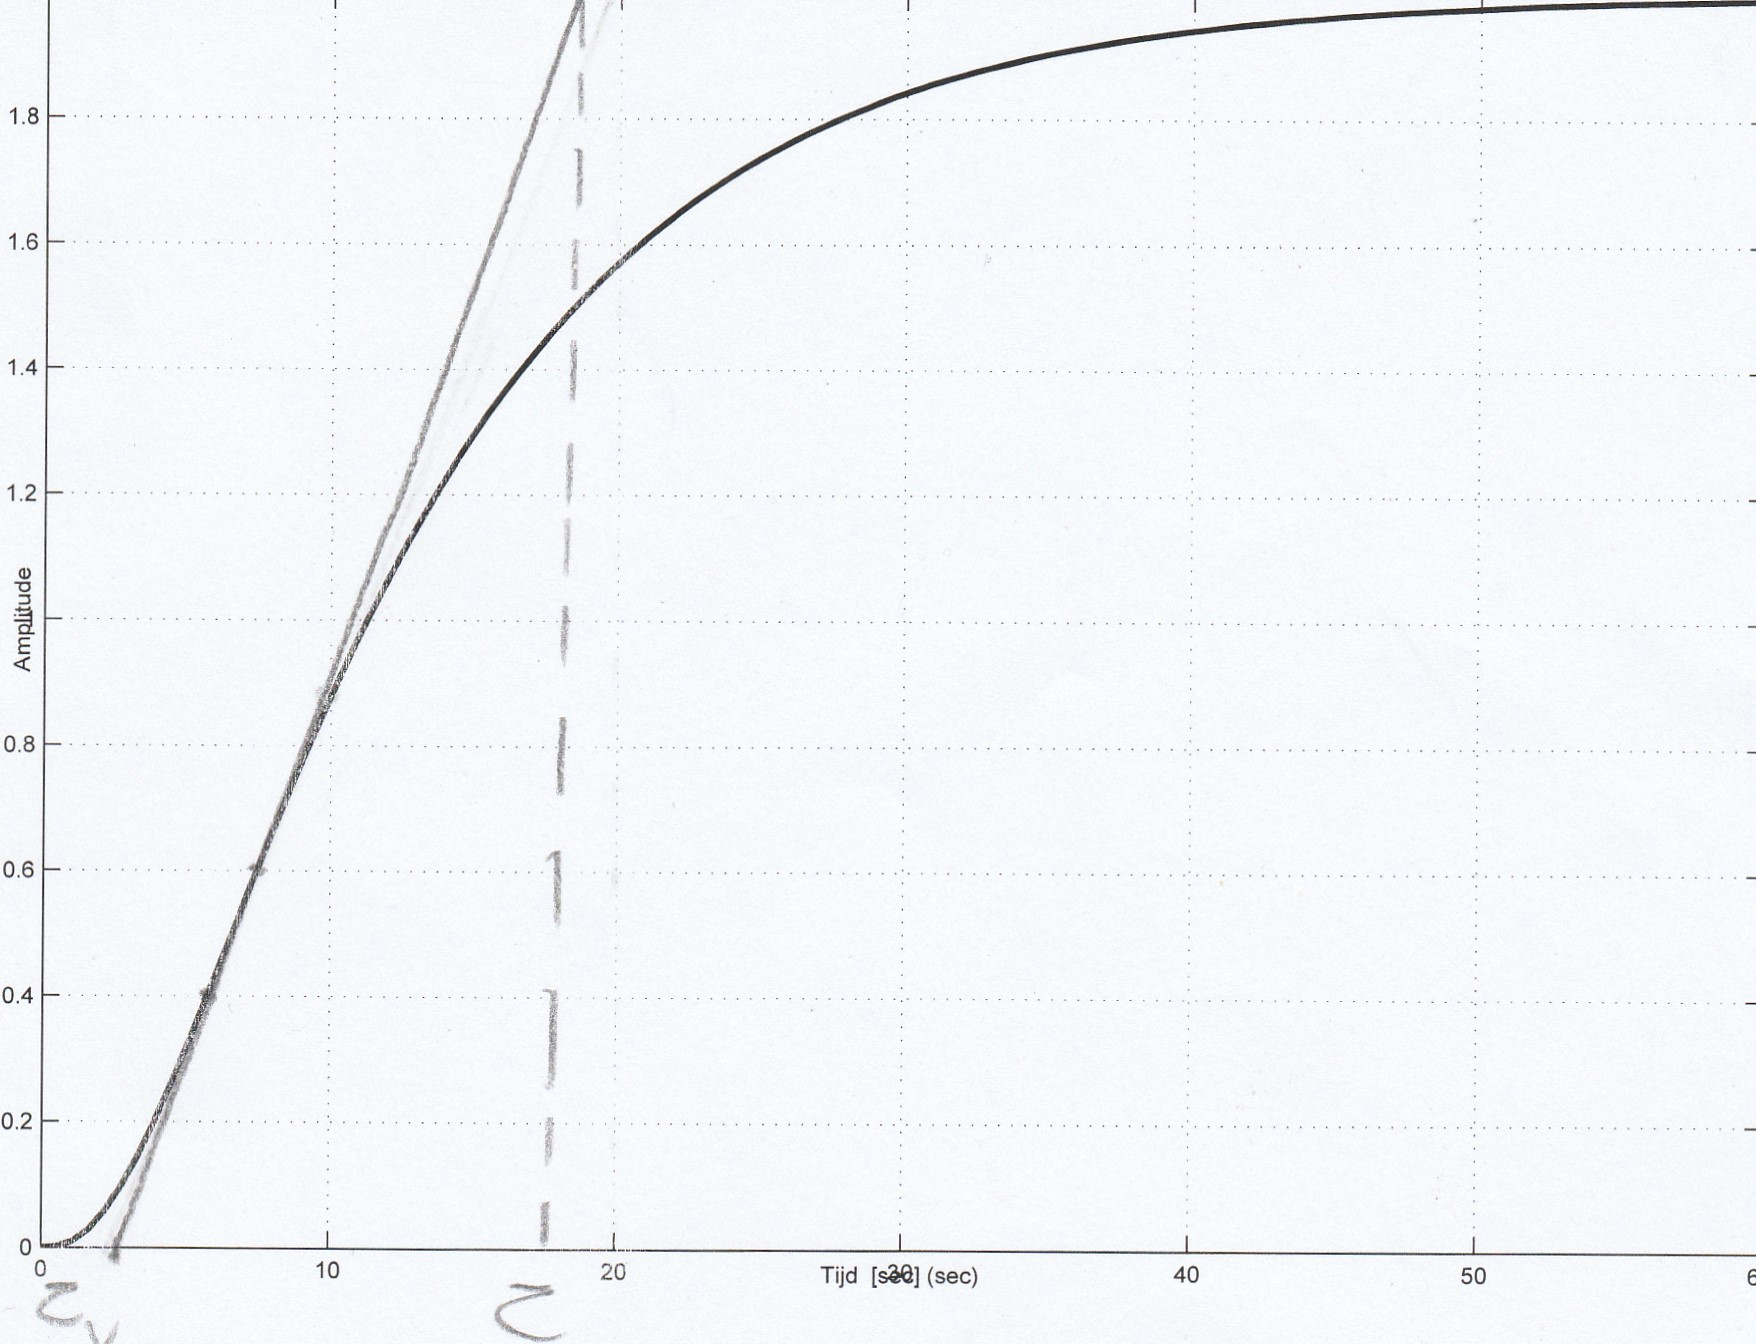
\includegraphics[width=1\linewidth]{Labo1_1.jpg}
	\caption{Gebruikte werkmethode}
\end{figure}	
	
\newpage

\subsection{Bepaal de gepaste regelaars voor een regeling hetzij storing met 20\% doorschot}

\begin{table}[!h]
\begin{large}
\centering
\resizebox{\columnwidth}{!}{
	\begin{tabular}{p{0.5\linewidth} p{0.5\linewidth}}
	$\frac{\tau}{\tau\textsubscript{v}} = \frac{14,8s}{2,4s} = 5,92$ & $3,3 < PID < 7,4 \rightarrow$ dus we gebruiken een PID regelaar \\ [3ex]
	Regelaar & Storing \\
	$K\textsubscript{R} = 0,95 * \frac{1}{K\textsubscript{p}} * \frac{\tau}{\tau\textsubscript{v}} = 2,812$ & $K\textsubscript{R} = 1,2 * \frac{1}{K\textsubscript{p}} * \frac{\tau}{\tau\textsubscript{v}} = 3,552$ \\
	$\tau\textsubscript{i} = 1,35\tau = 19,98s$ & $\tau\textsubscript{i} = 2\tau = 4,8s$ \\
	$\tau\textsubscript{d} = 0,47\tau\textsubscript{v} = 1,128s$ & $\tau\textsubscript{d} = 0,42\tau\textsubscript{v} = 1,008s$ \\
	\end{tabular}
}
\end{large}
\end{table}
Deze formules komen uit de tabel 5.1 uit de cursus voor een systeem met minimale oscillatieduur en 20\% doorschot.

\subsection{Simuleer de stapweergave van het geïdentificeerd systeem in open lus en vergelijk dit met de stapweergave van het ongekend systeem. Beoordeel de kwaliteit van de benadering.}

\begin{figure}[!h]
	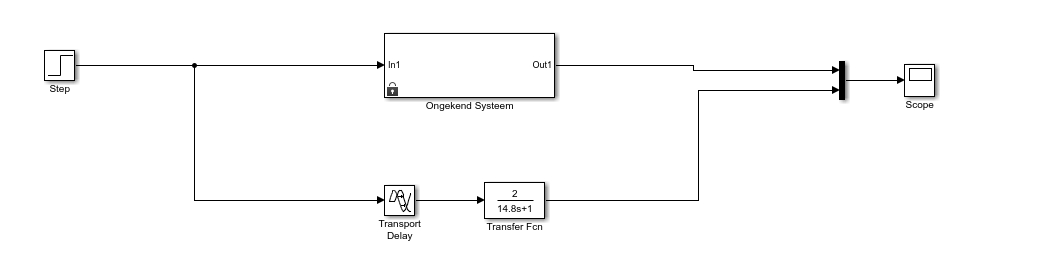
\includegraphics[width=1\linewidth]{Labo1_3_systeem.jpg}
	\caption{Figuur van het gebruikte simulink schema}
\end{figure}

\begin{figure}[!h]
	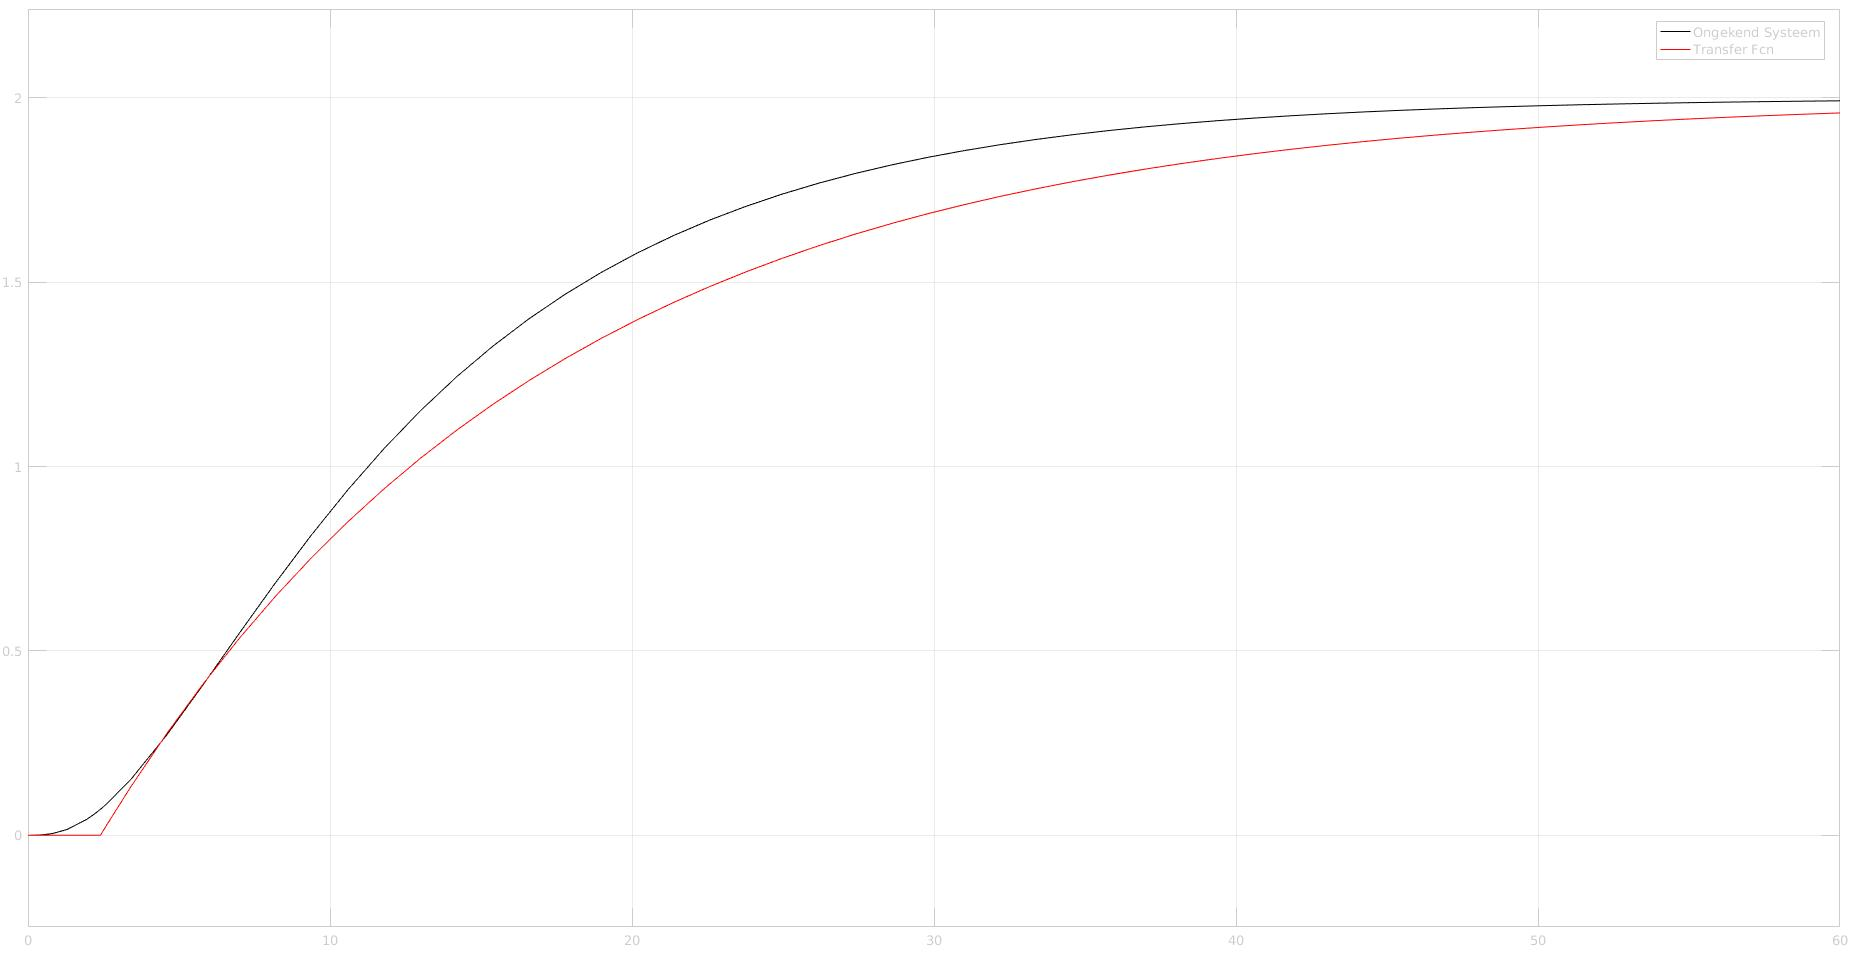
\includegraphics[width=1\linewidth]{Labo1_3_scoop.jpg}
	\caption{Simulatie van het onbekende en berekende systeem}
	\label{fig:scoop3.1}
\end{figure}

\newpage

Figuur \ref{fig:scoop3.1} toont ons de simulatie van het onbekende systeem en het berekende model. In deze figuur is de zwarte figuur het onbekende systeem en de rode figuur onze benaderend model. \\
Uit deze simulatie kunnen we besluiten dat onze dode tijd vrij goed lijkt te kloppen maar dat de benaderende simulatie wel trager verloopt als het onbekende systeem. We kunnen dan ook besluiten dat $\tau$ kleiner zal moeten zijn om een betere overeenkomst te bekomen. \\
Als we iteratief naar deze $\tau$ zouden toewerken, dit wil zeggen een steeds kleinere $\tau$ nemen tot dat deze lijkt te kloppen, zouden we op ongeveer $\tau = 12$ uitkomen. Het resultaat hiervan zien we in figuur \ref{fig:scoop3.2}.

\begin{figure}[!h]
	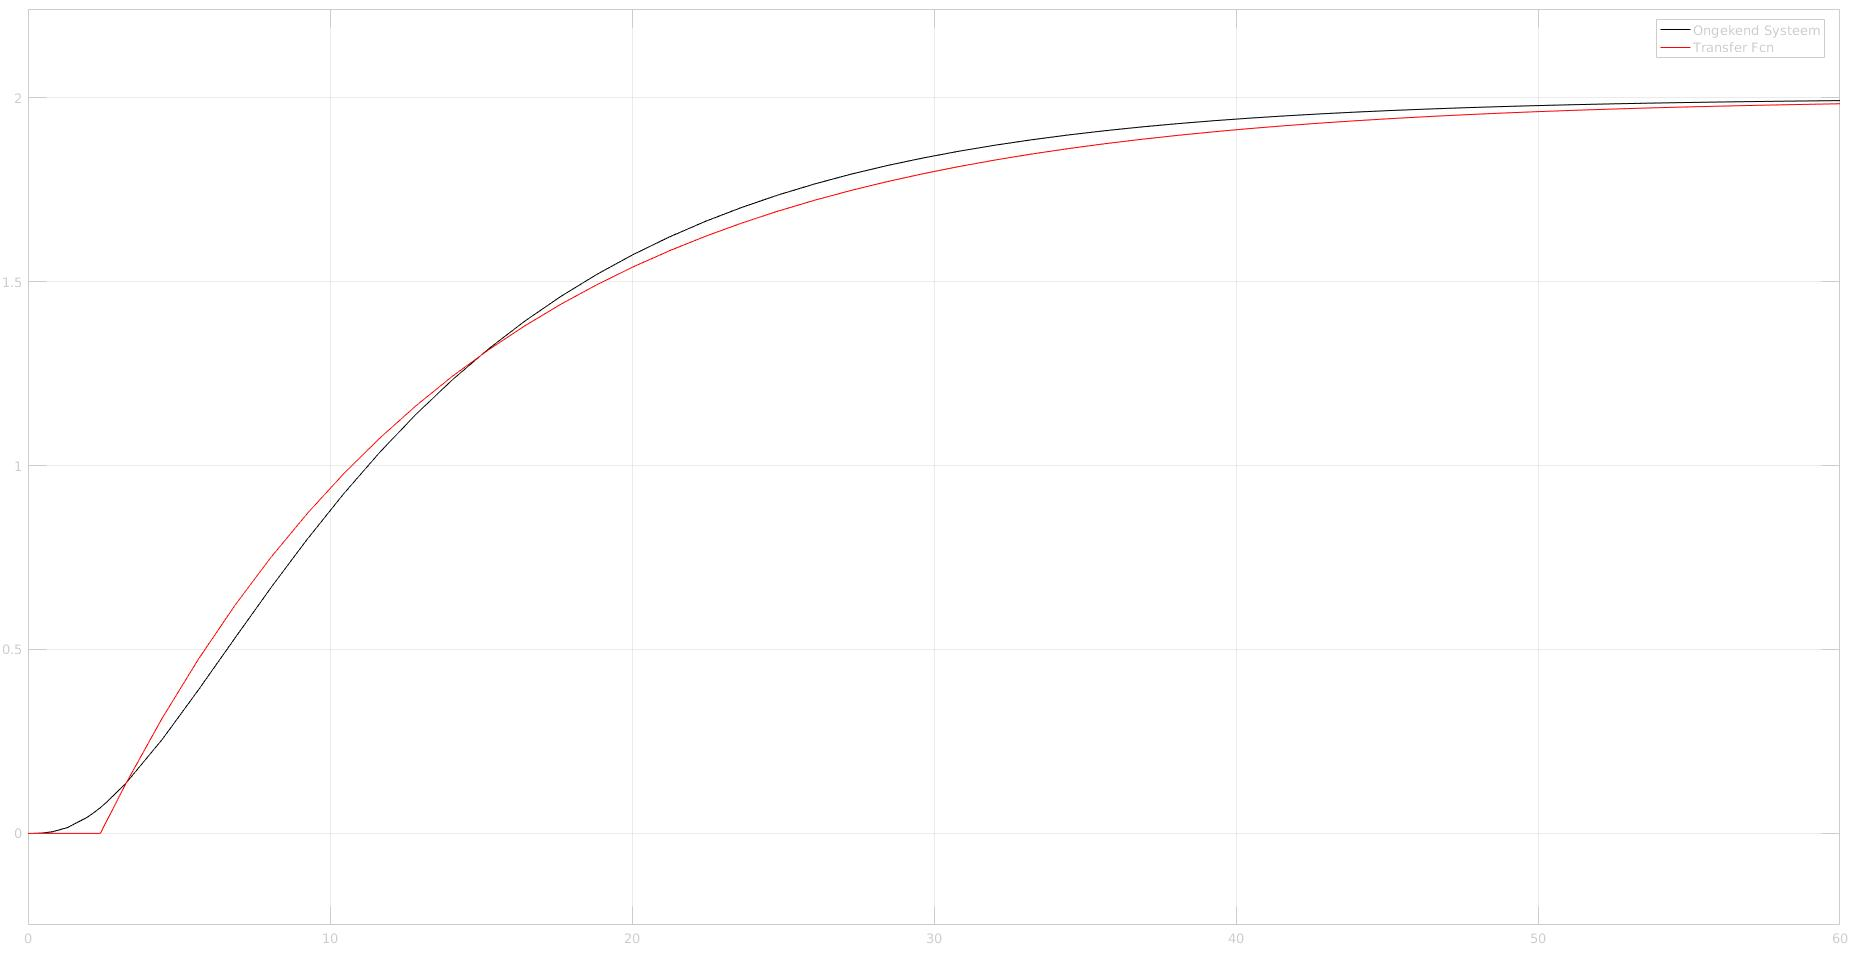
\includegraphics[width=0.9\linewidth]{Labo1_3_scoop2.jpg}
	\caption{Simulatie van het onbekende en berekende systeem na iteratief aanpassen van $\tau$}
	\label{fig:scoop3.2}
\end{figure}

\newpage

\subsection{Simuleer de reactie van het systeem in gesloten lus met toepassing van de regelaars en vergelijk weerom met de stapweergave van het werkelijk systeem bij deze regelaarsinstelling}

\begin{figure}[!h]
	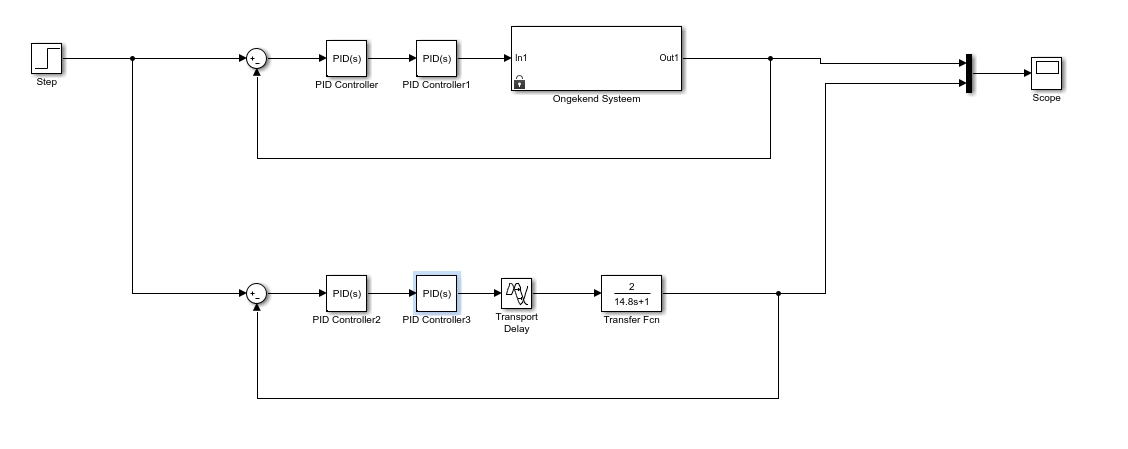
\includegraphics[width=1\linewidth]{Labo1_4_systeem.jpg}
	\caption{Figuur van het gebruikte simulink schema met regelaar}
\end{figure}

\begin{figure}[!h]
	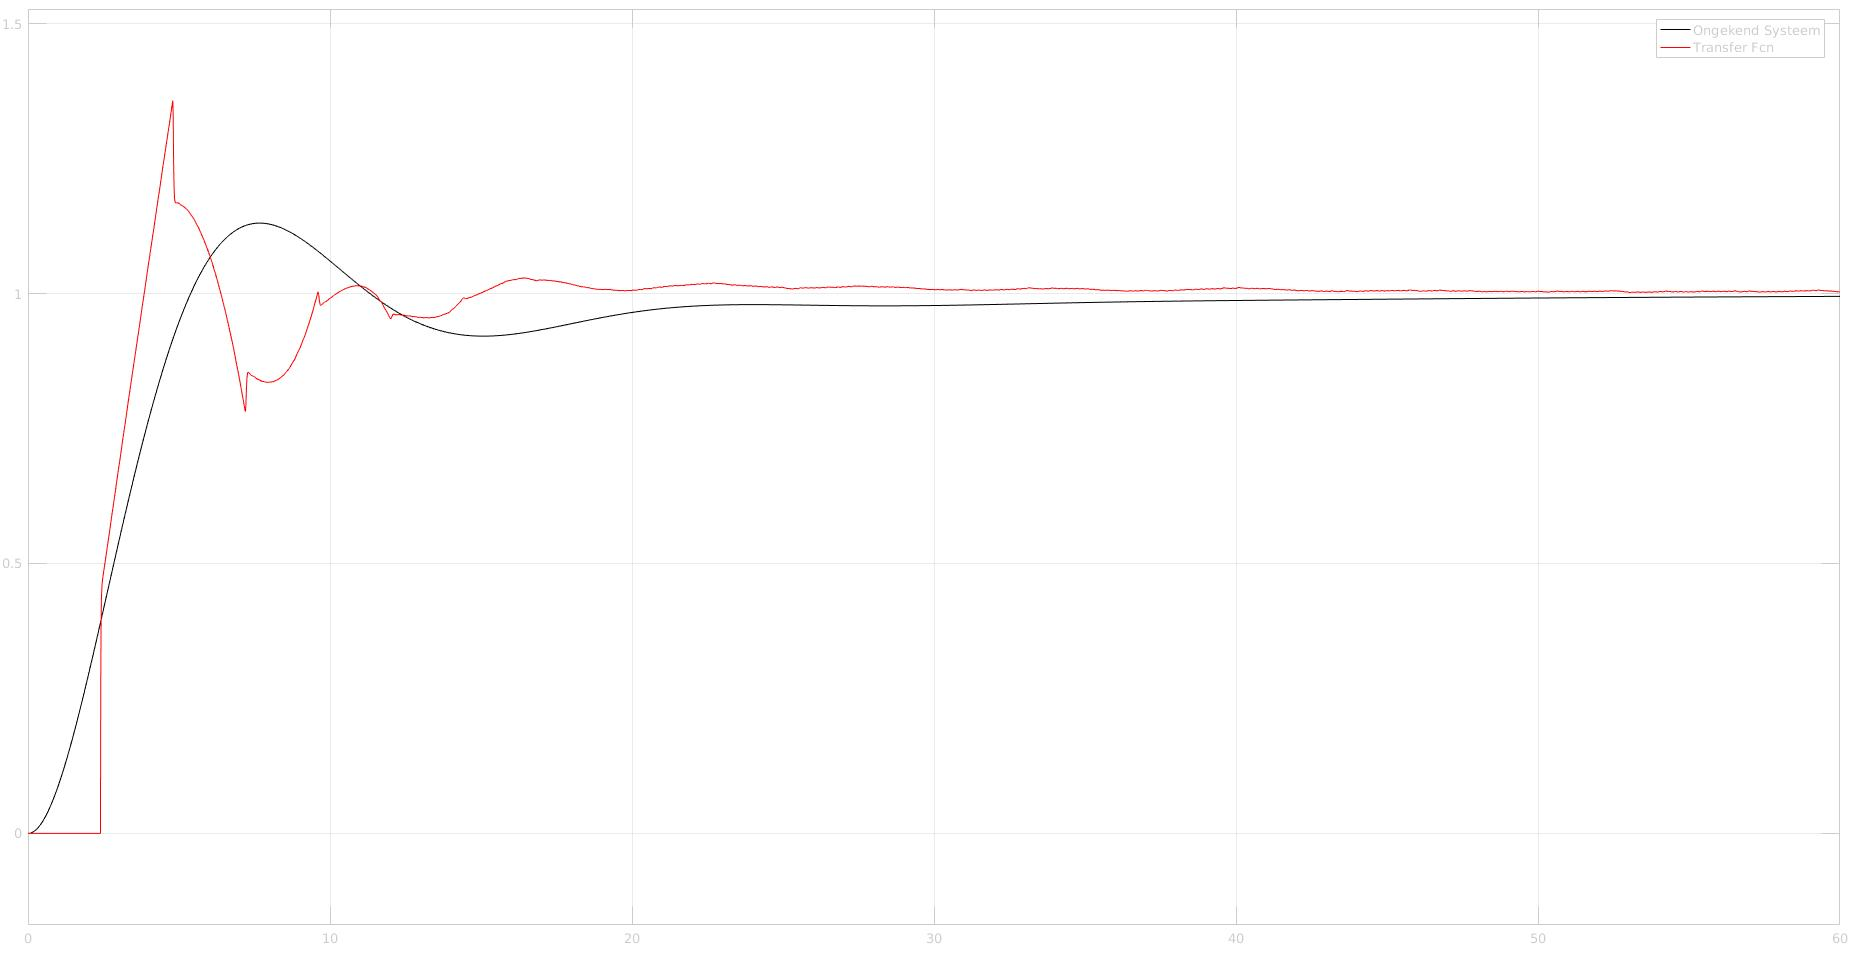
\includegraphics[width=1\linewidth]{Labo1_4_scoop.jpg}
	\caption{Simulatie van het onbekende en berekende systeem met regelaar}
	\label{fig:scoop4.1}
\end{figure}

Figuur \ref{fig:scoop4.1} geeft de simulatie weer. De gebruikte kleuren zijn dezelfde als in de vorige figuren. De regelaar bij het onbekende systeem zorgt voor minder oscillaties dan bij het berekende systeem, wat nogmaals wijst dat ons berekende systeem niet perfect overeenkomt. Ook heeft het berekende systeem een paar rare uitschieters die niet in het originele systeem terug te vinden zijn.

\newpage

\section{\underline{Opgave 2}}

\subsection{Identificeer het ongekend systeem door toepassing van de methode van Strejec.}

Strejec gebruikt de transferfunctie : $H(p) = \frac{K\textsubscript{p}}{(1+\tau p)^n}$. De onbekende hierbij zijn n en $\tau$ en deze vinden we via de nomogram overdrachtsfuncties. \\ [2ex]
$\tau\textsubscript{v}' = 2,4s$ \\
$\tau' = 14,8s$ \\ [2ex]
$\frac{\tau\textsubscript{v}'}{\tau'} = 0,16$ \\
$K\textsubscript{p} = 2$ \\

Uit figuur \ref{fig:fig2_1} kunnen we aflezen dat $n = 2,5$ en dat $\tau = 4,5$. \\
De transferfunctie wordt dan : $H(p) = \frac{2}{(1+4,5p)^2,5}$.

\subsection{Bepaal de coëfficienten van een gepaste regelaar (20\% doorschot)}

Omdat simulink alleen n als gehele getallen kan nemen en 2,5 geen geheel getal is, doen we ook alle berekeningen voor n = 2 en n = 3.

\begin{table}[!h]
\begin{large}
\centering
\resizebox{\columnwidth}{!}{
		\begin{tabular}{p{0.1\linewidth} p{0.40\linewidth} p{0.20\linewidth} p{0.30\linewidth}}
		n = 2 & $\rightarrow \alpha = 1,9 + 0,1 * \frac{0,3}{1,5} = 1,92$ & $\rightarrow K = 1,10$ & $\rightarrow a = \frac{1,15}{\tau+} = 0,256$ \\[5ex]
		n = 2,5 & $\rightarrow \alpha = 1,8 + 0,1 * \frac{1,1}{1,5} = 1,873$ & $\rightarrow K = 0,8$ & $\rightarrow a = \frac{0,7}{\tau} = 0,156$ \\[5ex]
		n = 3 & $\rightarrow \alpha = 1,8 + 0,1 * \frac{0,3}{1,5} = 1,82$ & $\rightarrow K = 0,66$ & $\rightarrow a = \frac{0,5}{\tau} = 0,111$ \\
		\end{tabular}
}
\end{large}
\end{table}

Deze gegevens voor $a, K$ en $\alpha$ zijn gevonden door de figuren \ref{fig:fig2_2_1}, \ref{fig:fig2_2_2} en \ref{fig:fig2_2_3}. \\ 

n = 2 \\
$K = K\textsubscript{p}*K\textsubscript{r} = 2*K\textsubscript{r} \rightarrow K\textsubscript{r} = 0,55$ \\
$a = \frac{K\textsubscript{p}*K\textsubscript{r}}{\tau\textsubscript{i}} \rightarrow \tau\textsubscript{i} = \frac{K\textsubscript{p}*K\textsubscript{r}}{a} = 4,30$ \\ [3ex]

n = 2,5 \\
$K = K\textsubscript{p}*K\textsubscript{r} = 2*K\textsubscript{r} \rightarrow K\textsubscript{r} = 0,4$ \\
$a = \frac{K\textsubscript{p}*K\textsubscript{r}}{\tau\textsubscript{i}} \rightarrow \tau\textsubscript{i} = \frac{K\textsubscript{p}*K\textsubscript{r}}{a} = 5,13$ \\ [3ex]

n = 3 \\
$K = K\textsubscript{p}*K\textsubscript{r} = 2*K\textsubscript{r} \rightarrow K\textsubscript{r} = 0,33$ \\
$a = \frac{K\textsubscript{p}*K\textsubscript{r}}{\tau\textsubscript{i}} \rightarrow \tau\textsubscript{i} = \frac{K\textsubscript{p}*K\textsubscript{r}}{a} = 5,95$ \\

\begin{figure}[H]
	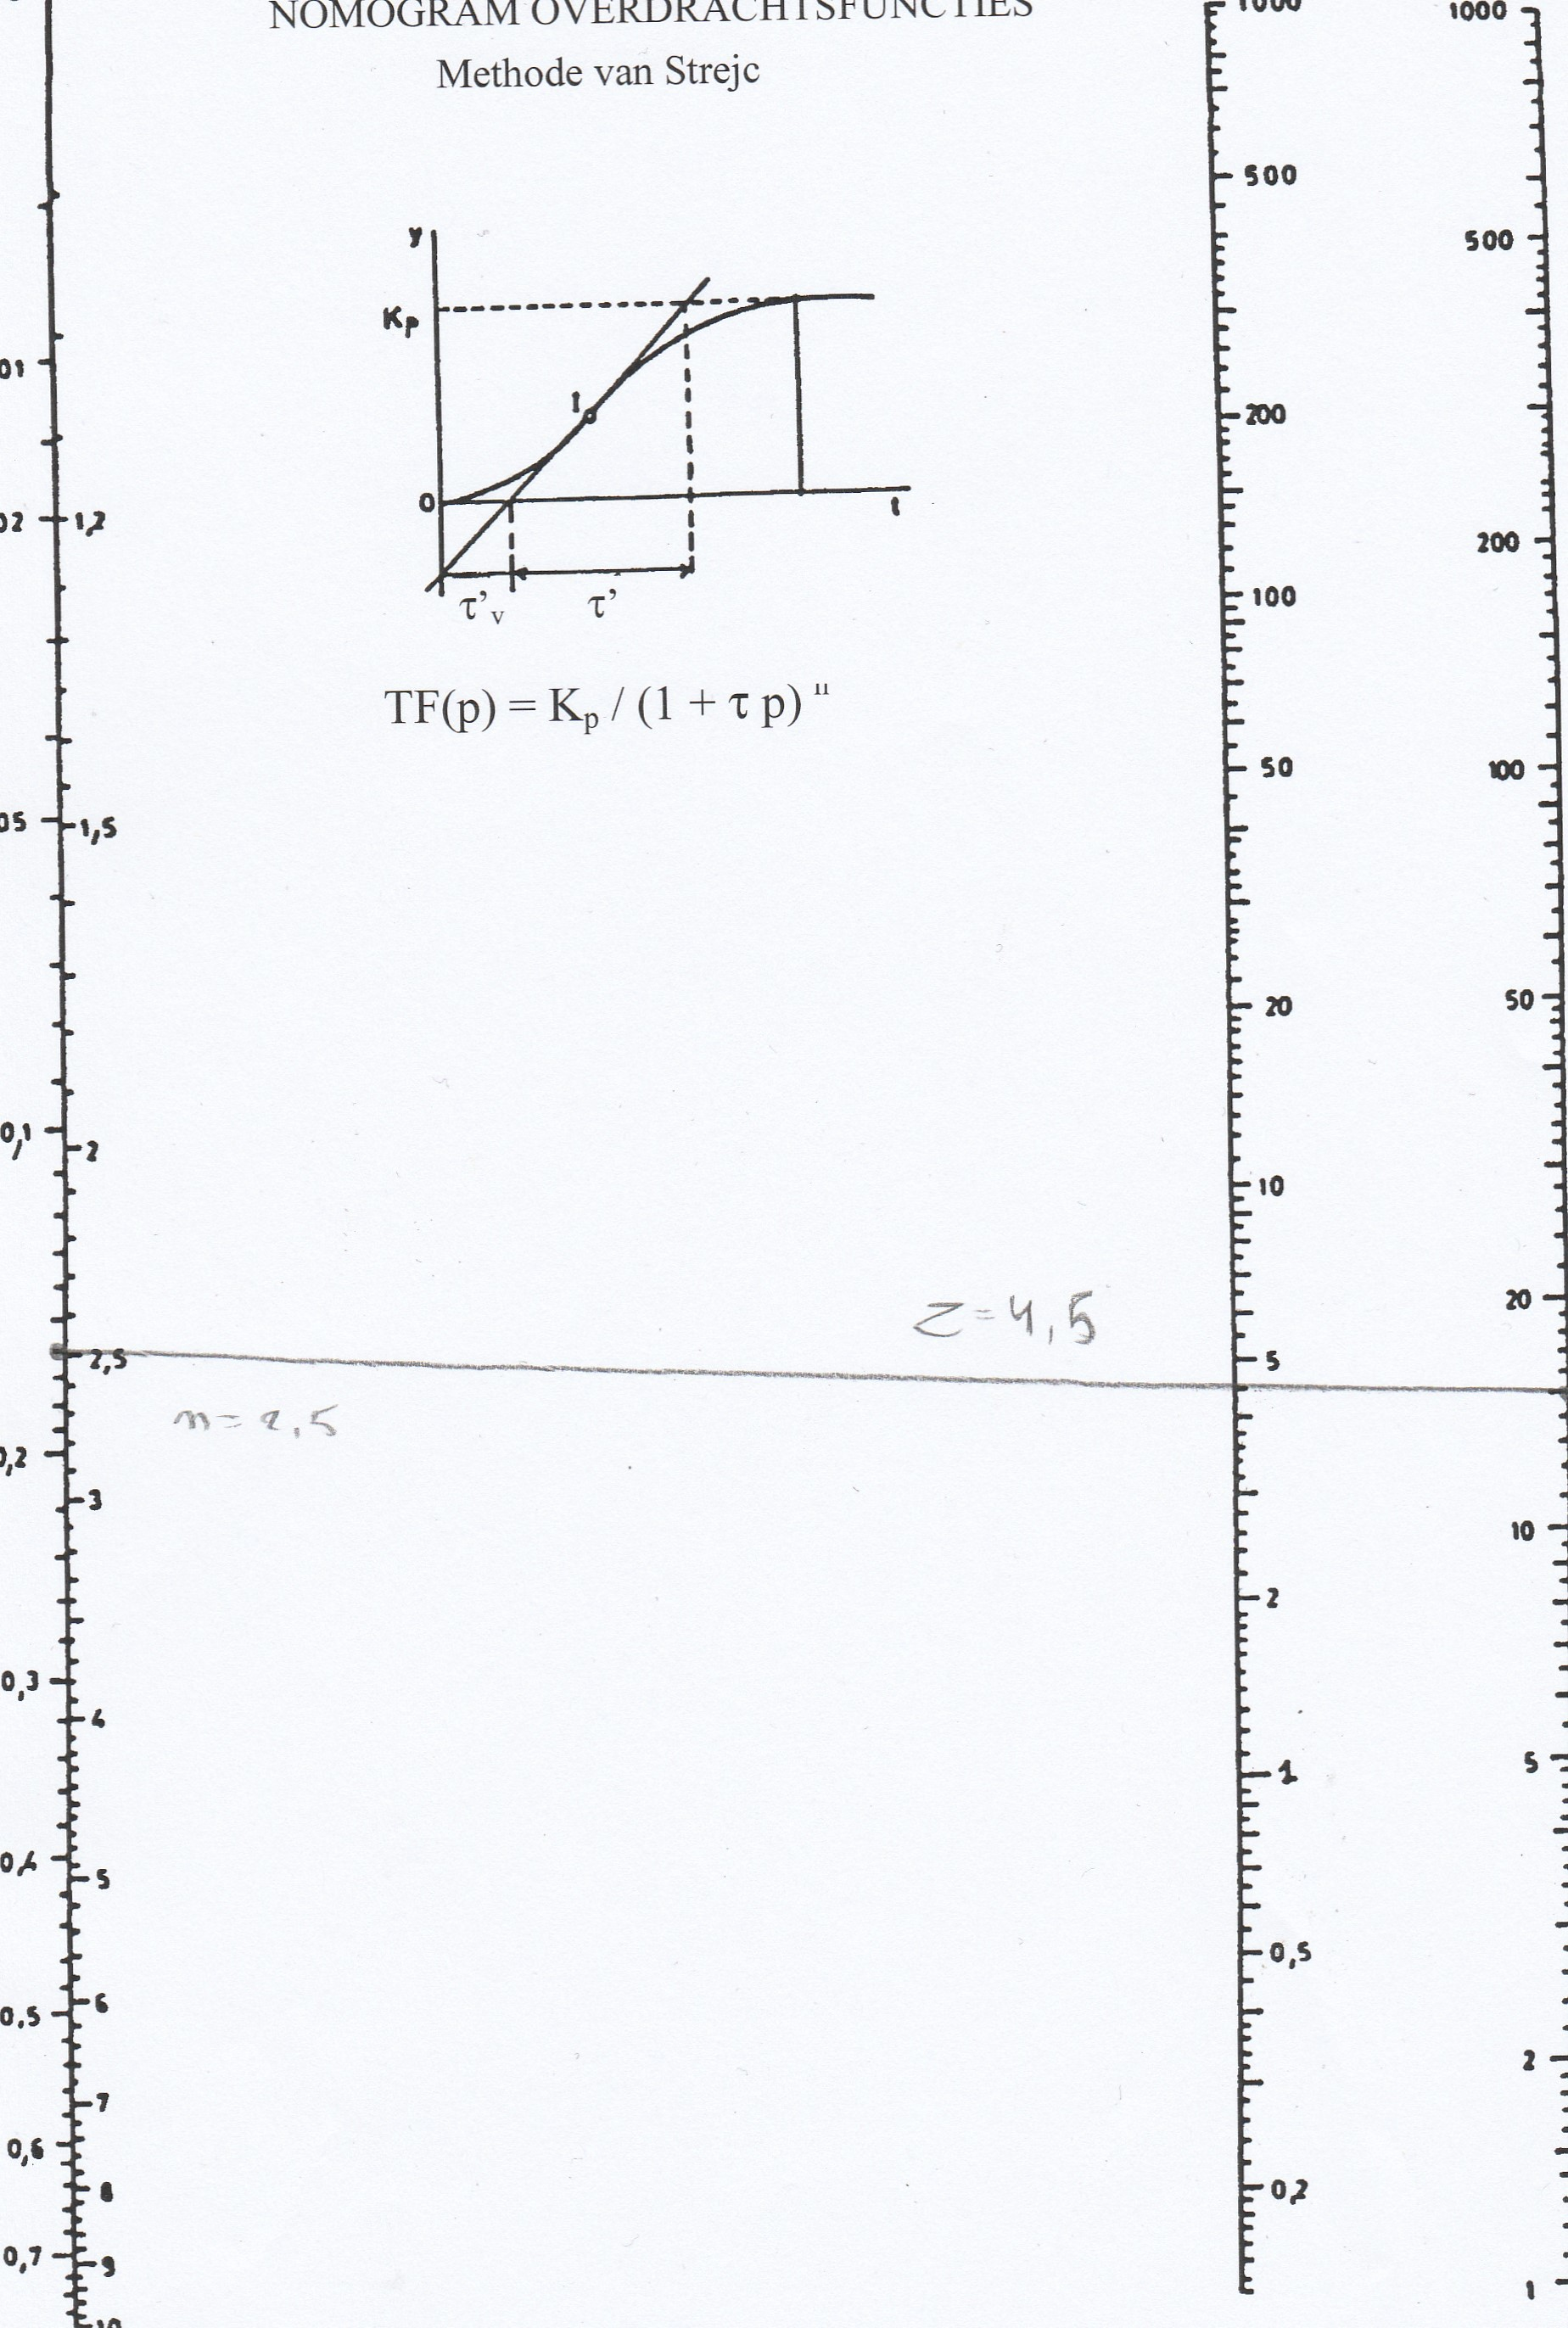
\includegraphics[width=1\linewidth]{Labo2_1.jpg}
	\caption{Nomogram overdrachtfuncties}
	\label{fig:fig2_1}
\end{figure}

\begin{figure}[H]	
	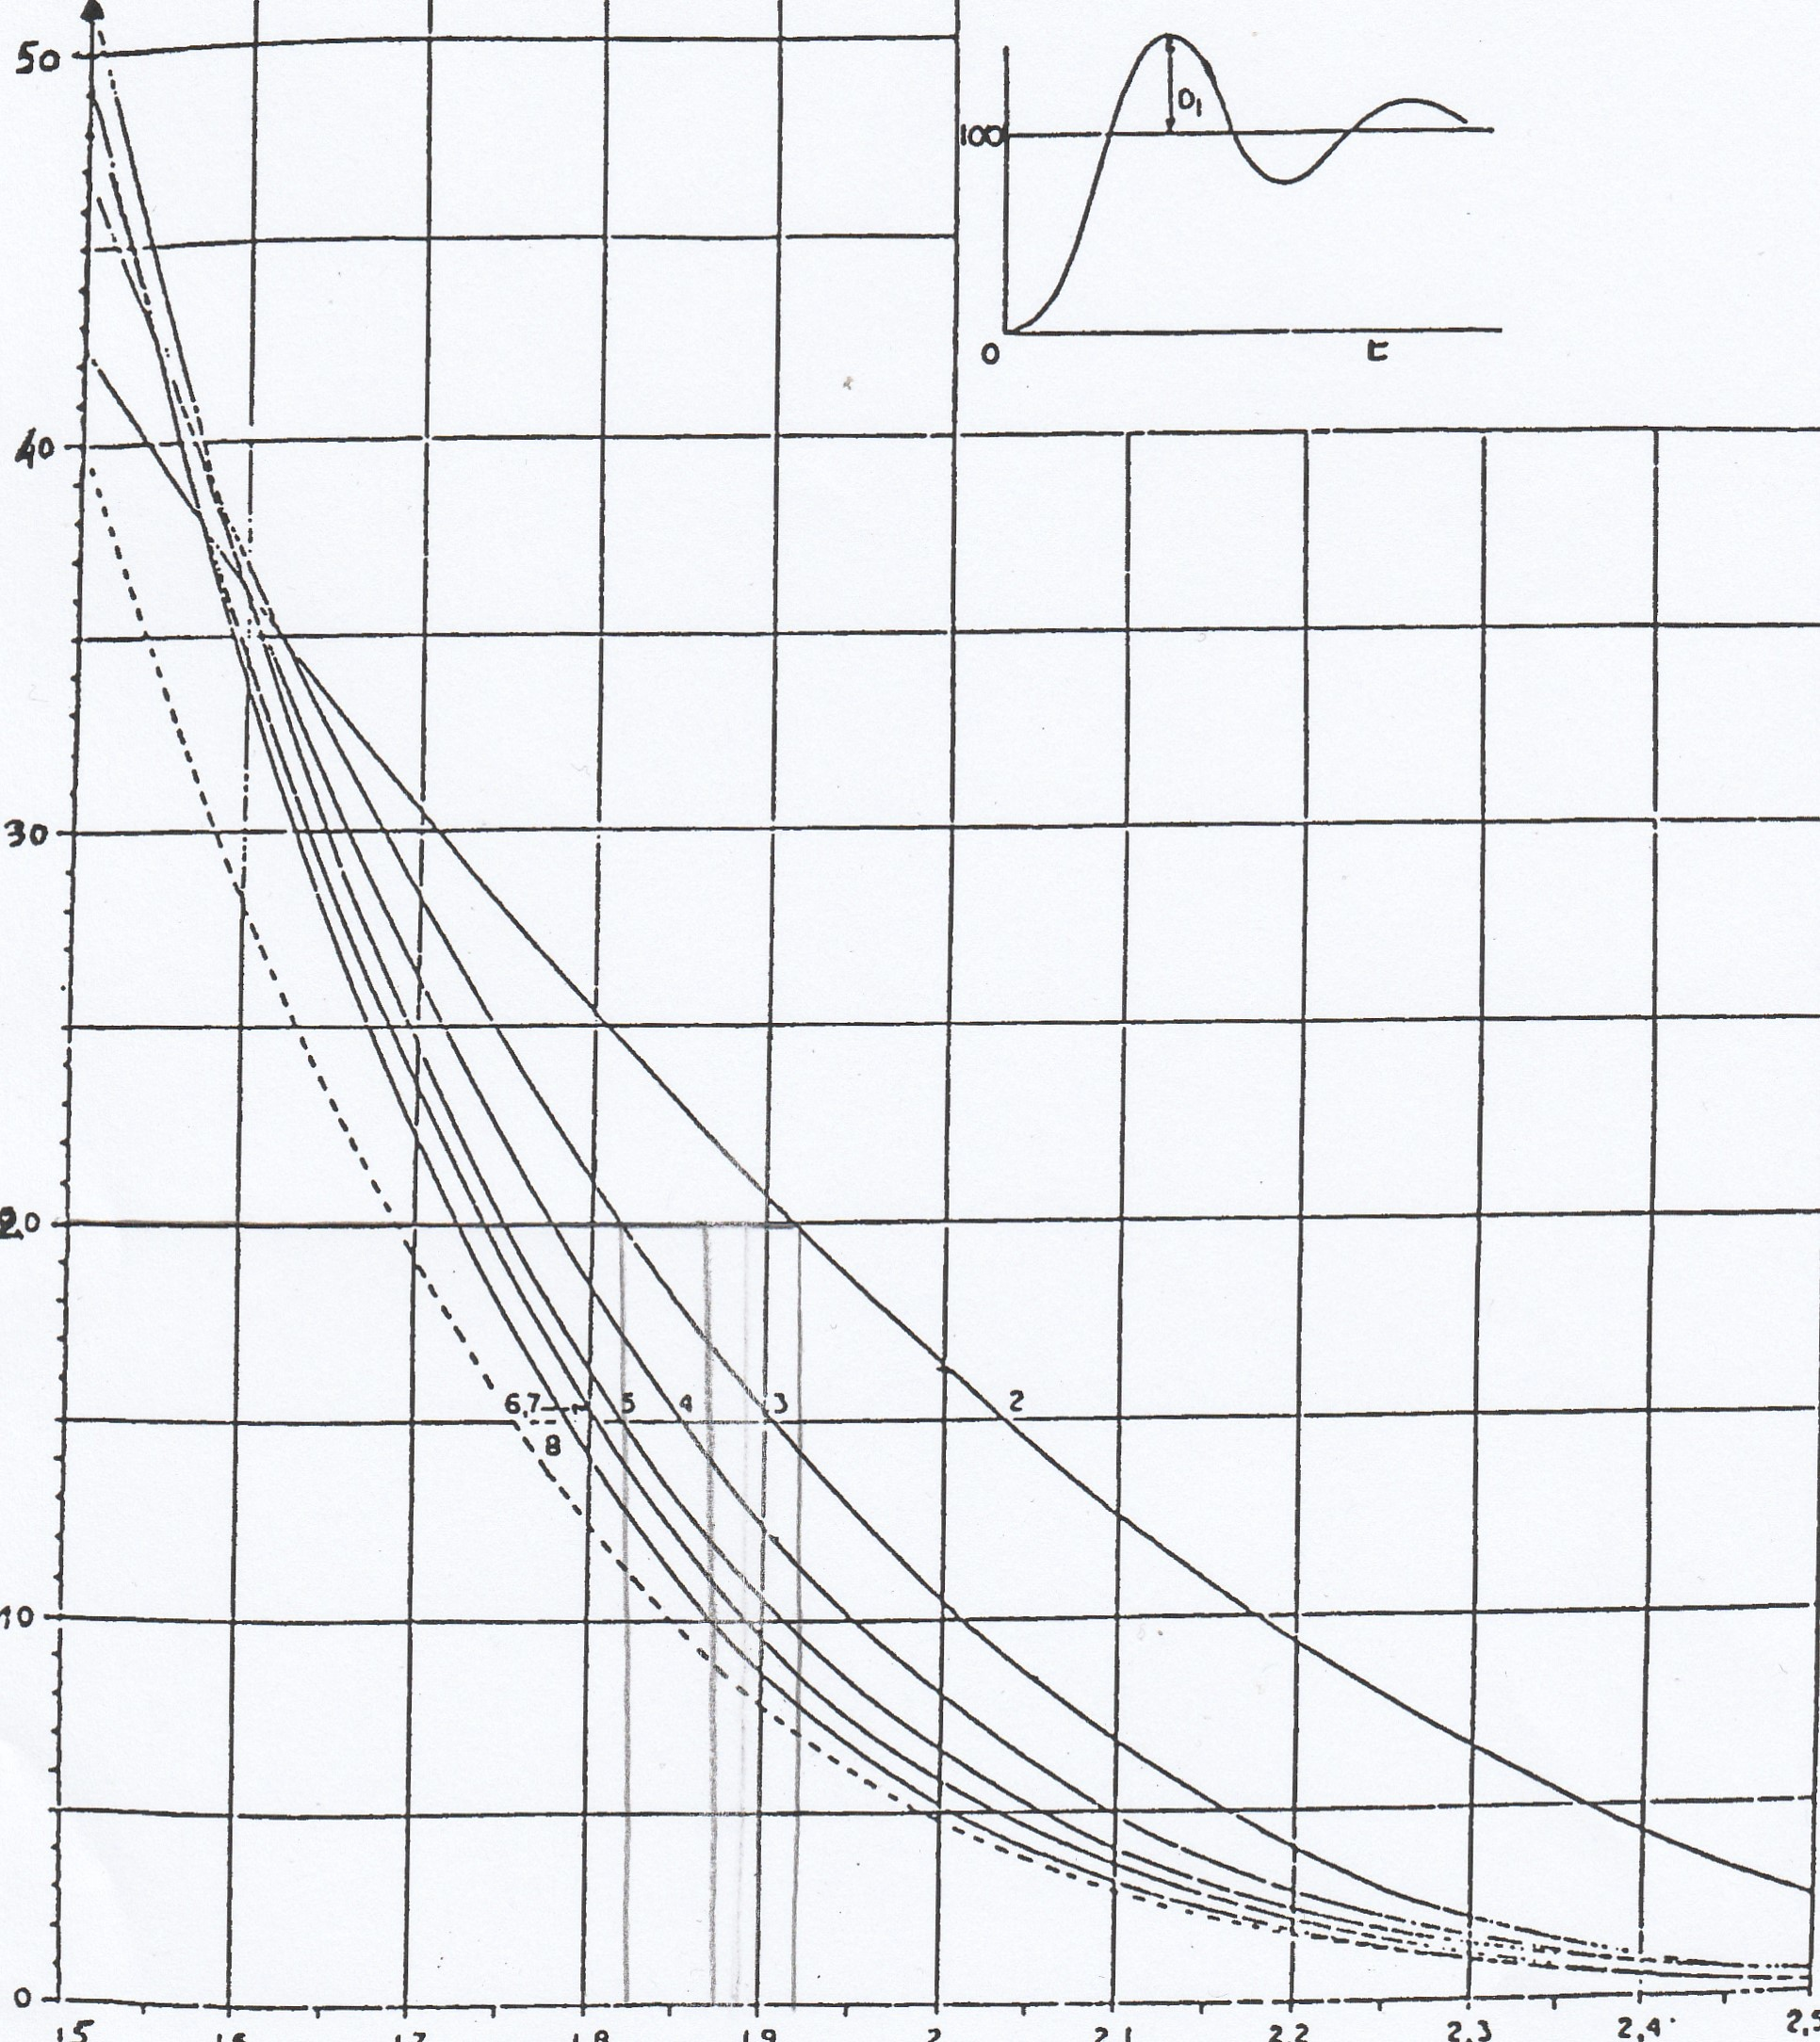
\includegraphics[width=1\linewidth]{Labo2_2_1.jpg}
	\caption{Doorschot met een PI-regelaar}
	\label{fig:fig2_2_1}
\end{figure}

\begin{figure}[H]
	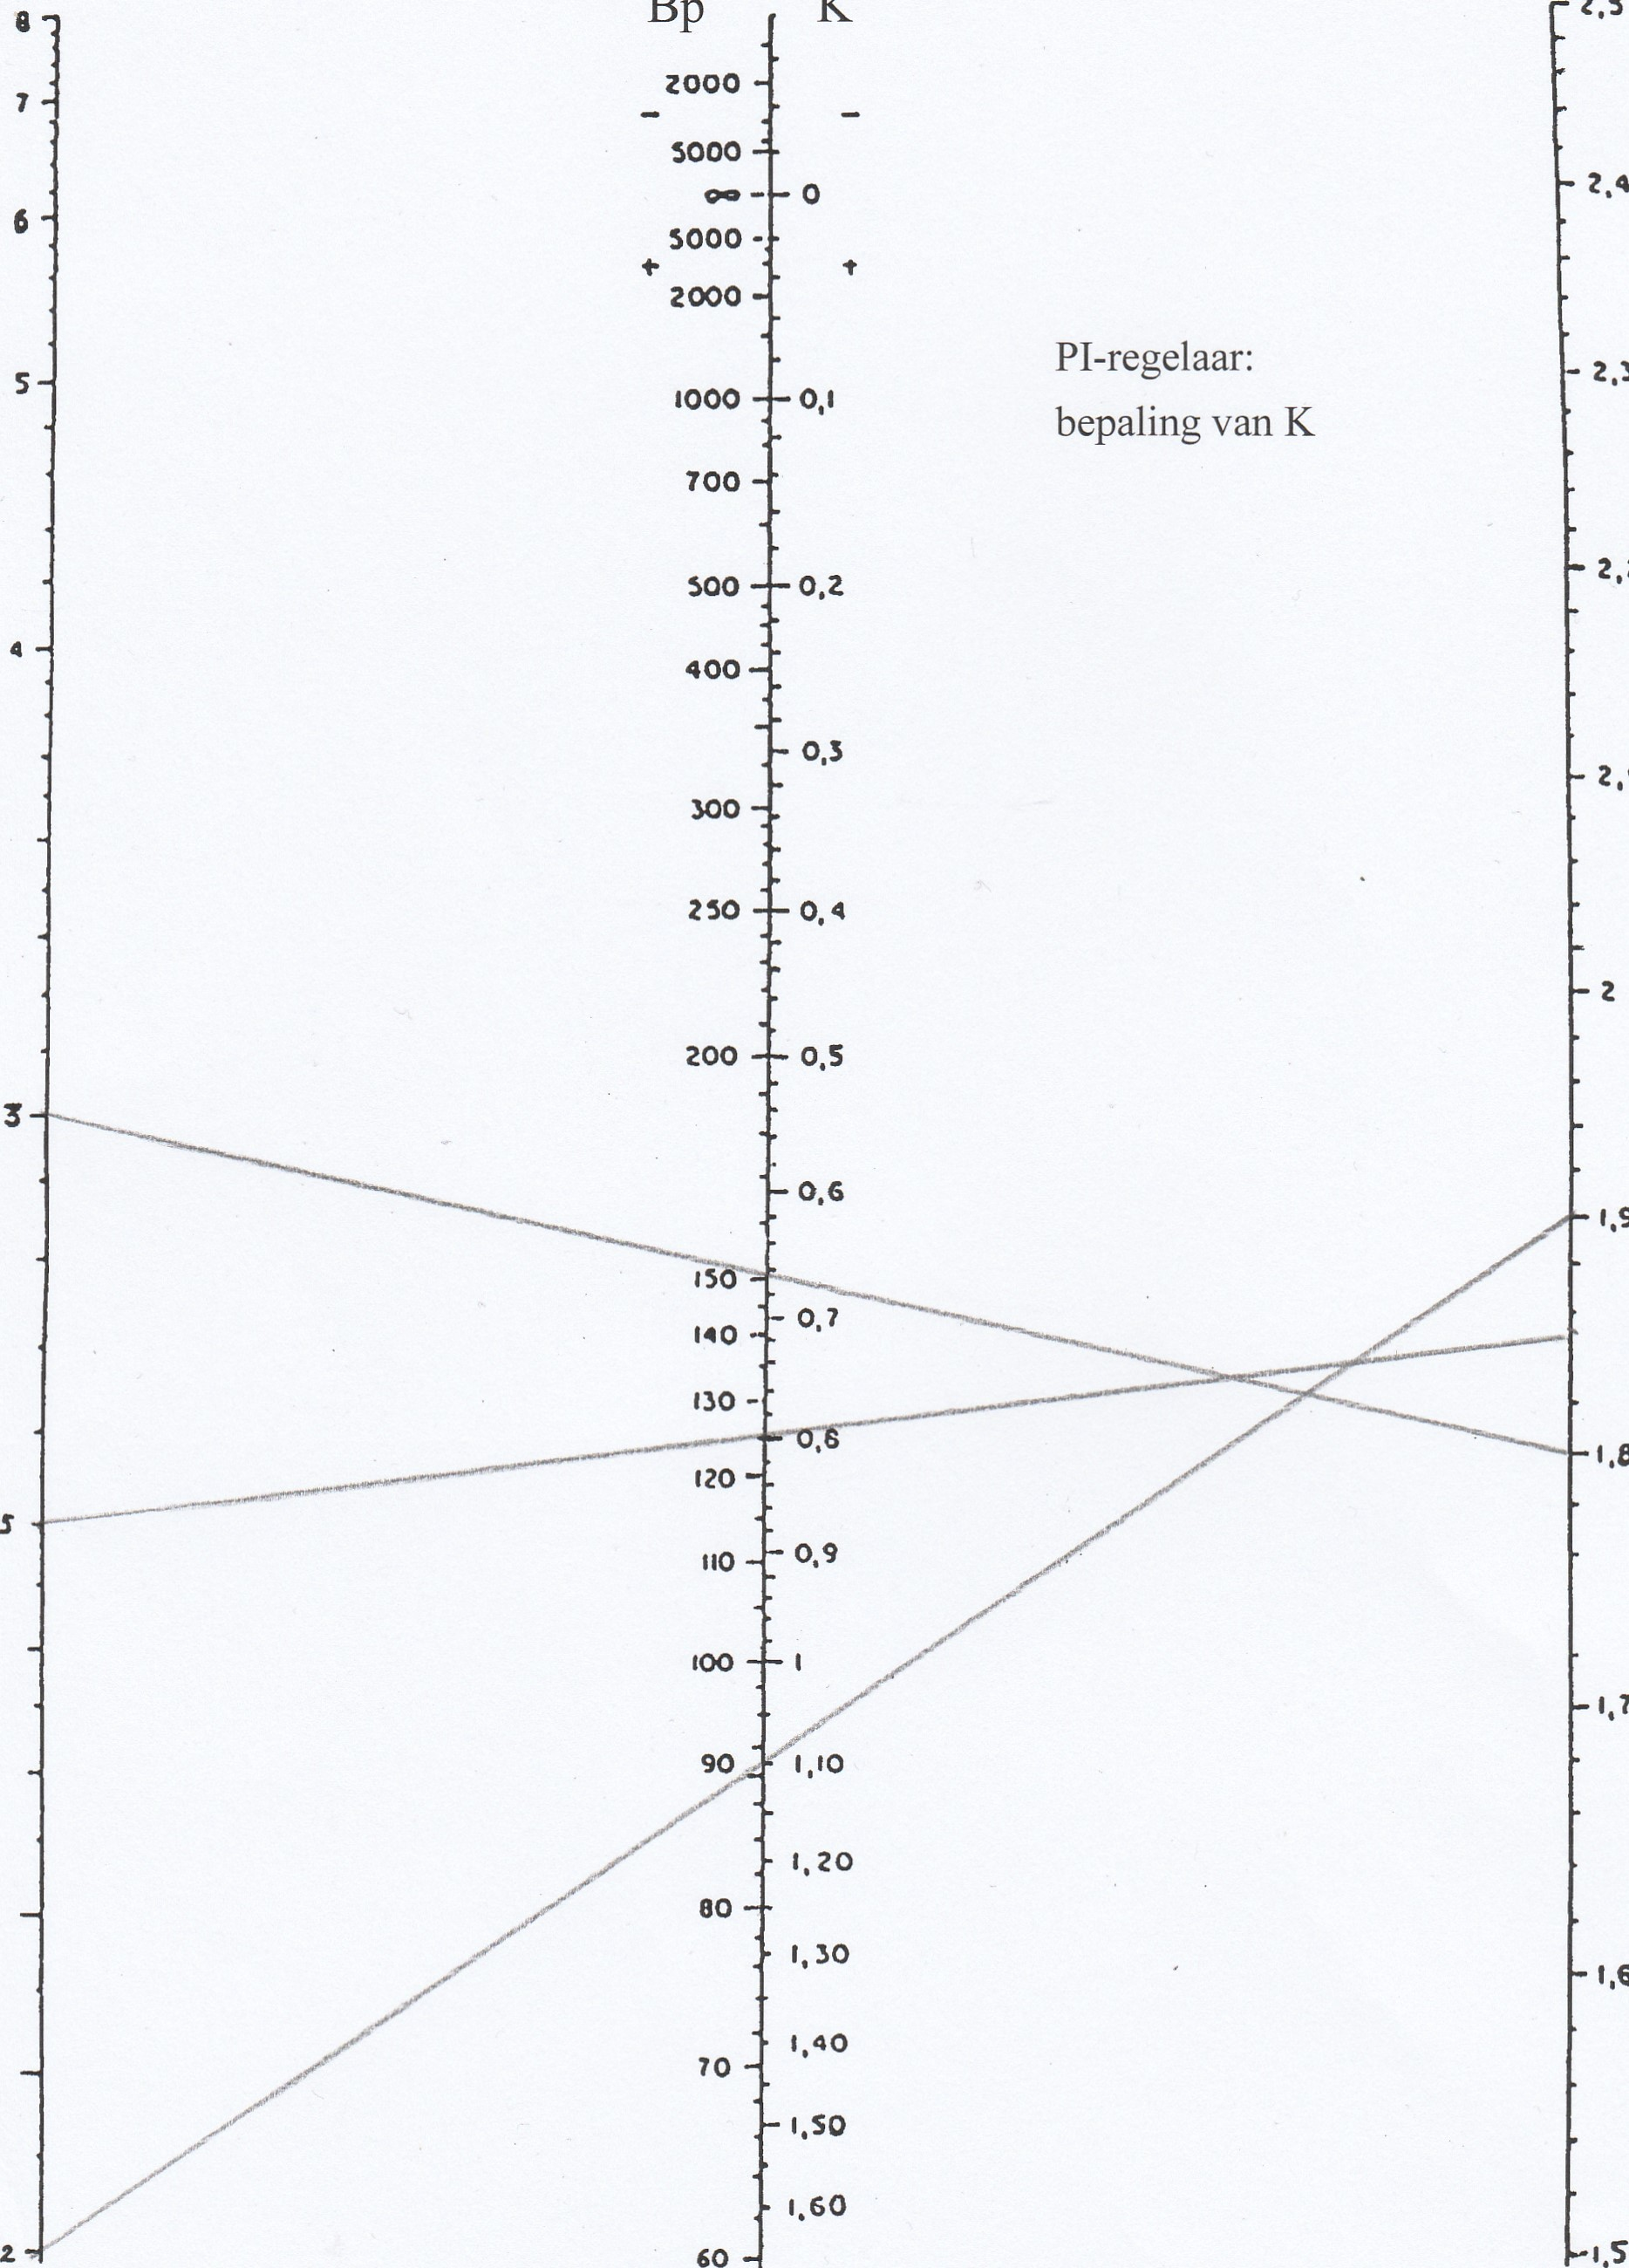
\includegraphics[width=1\linewidth]{Labo2_2_2.jpg}
	\caption{PI-regelaar: bepaling van K}
	\label{fig:fig2_2_2}
\end{figure}

\begin{figure}[H]
	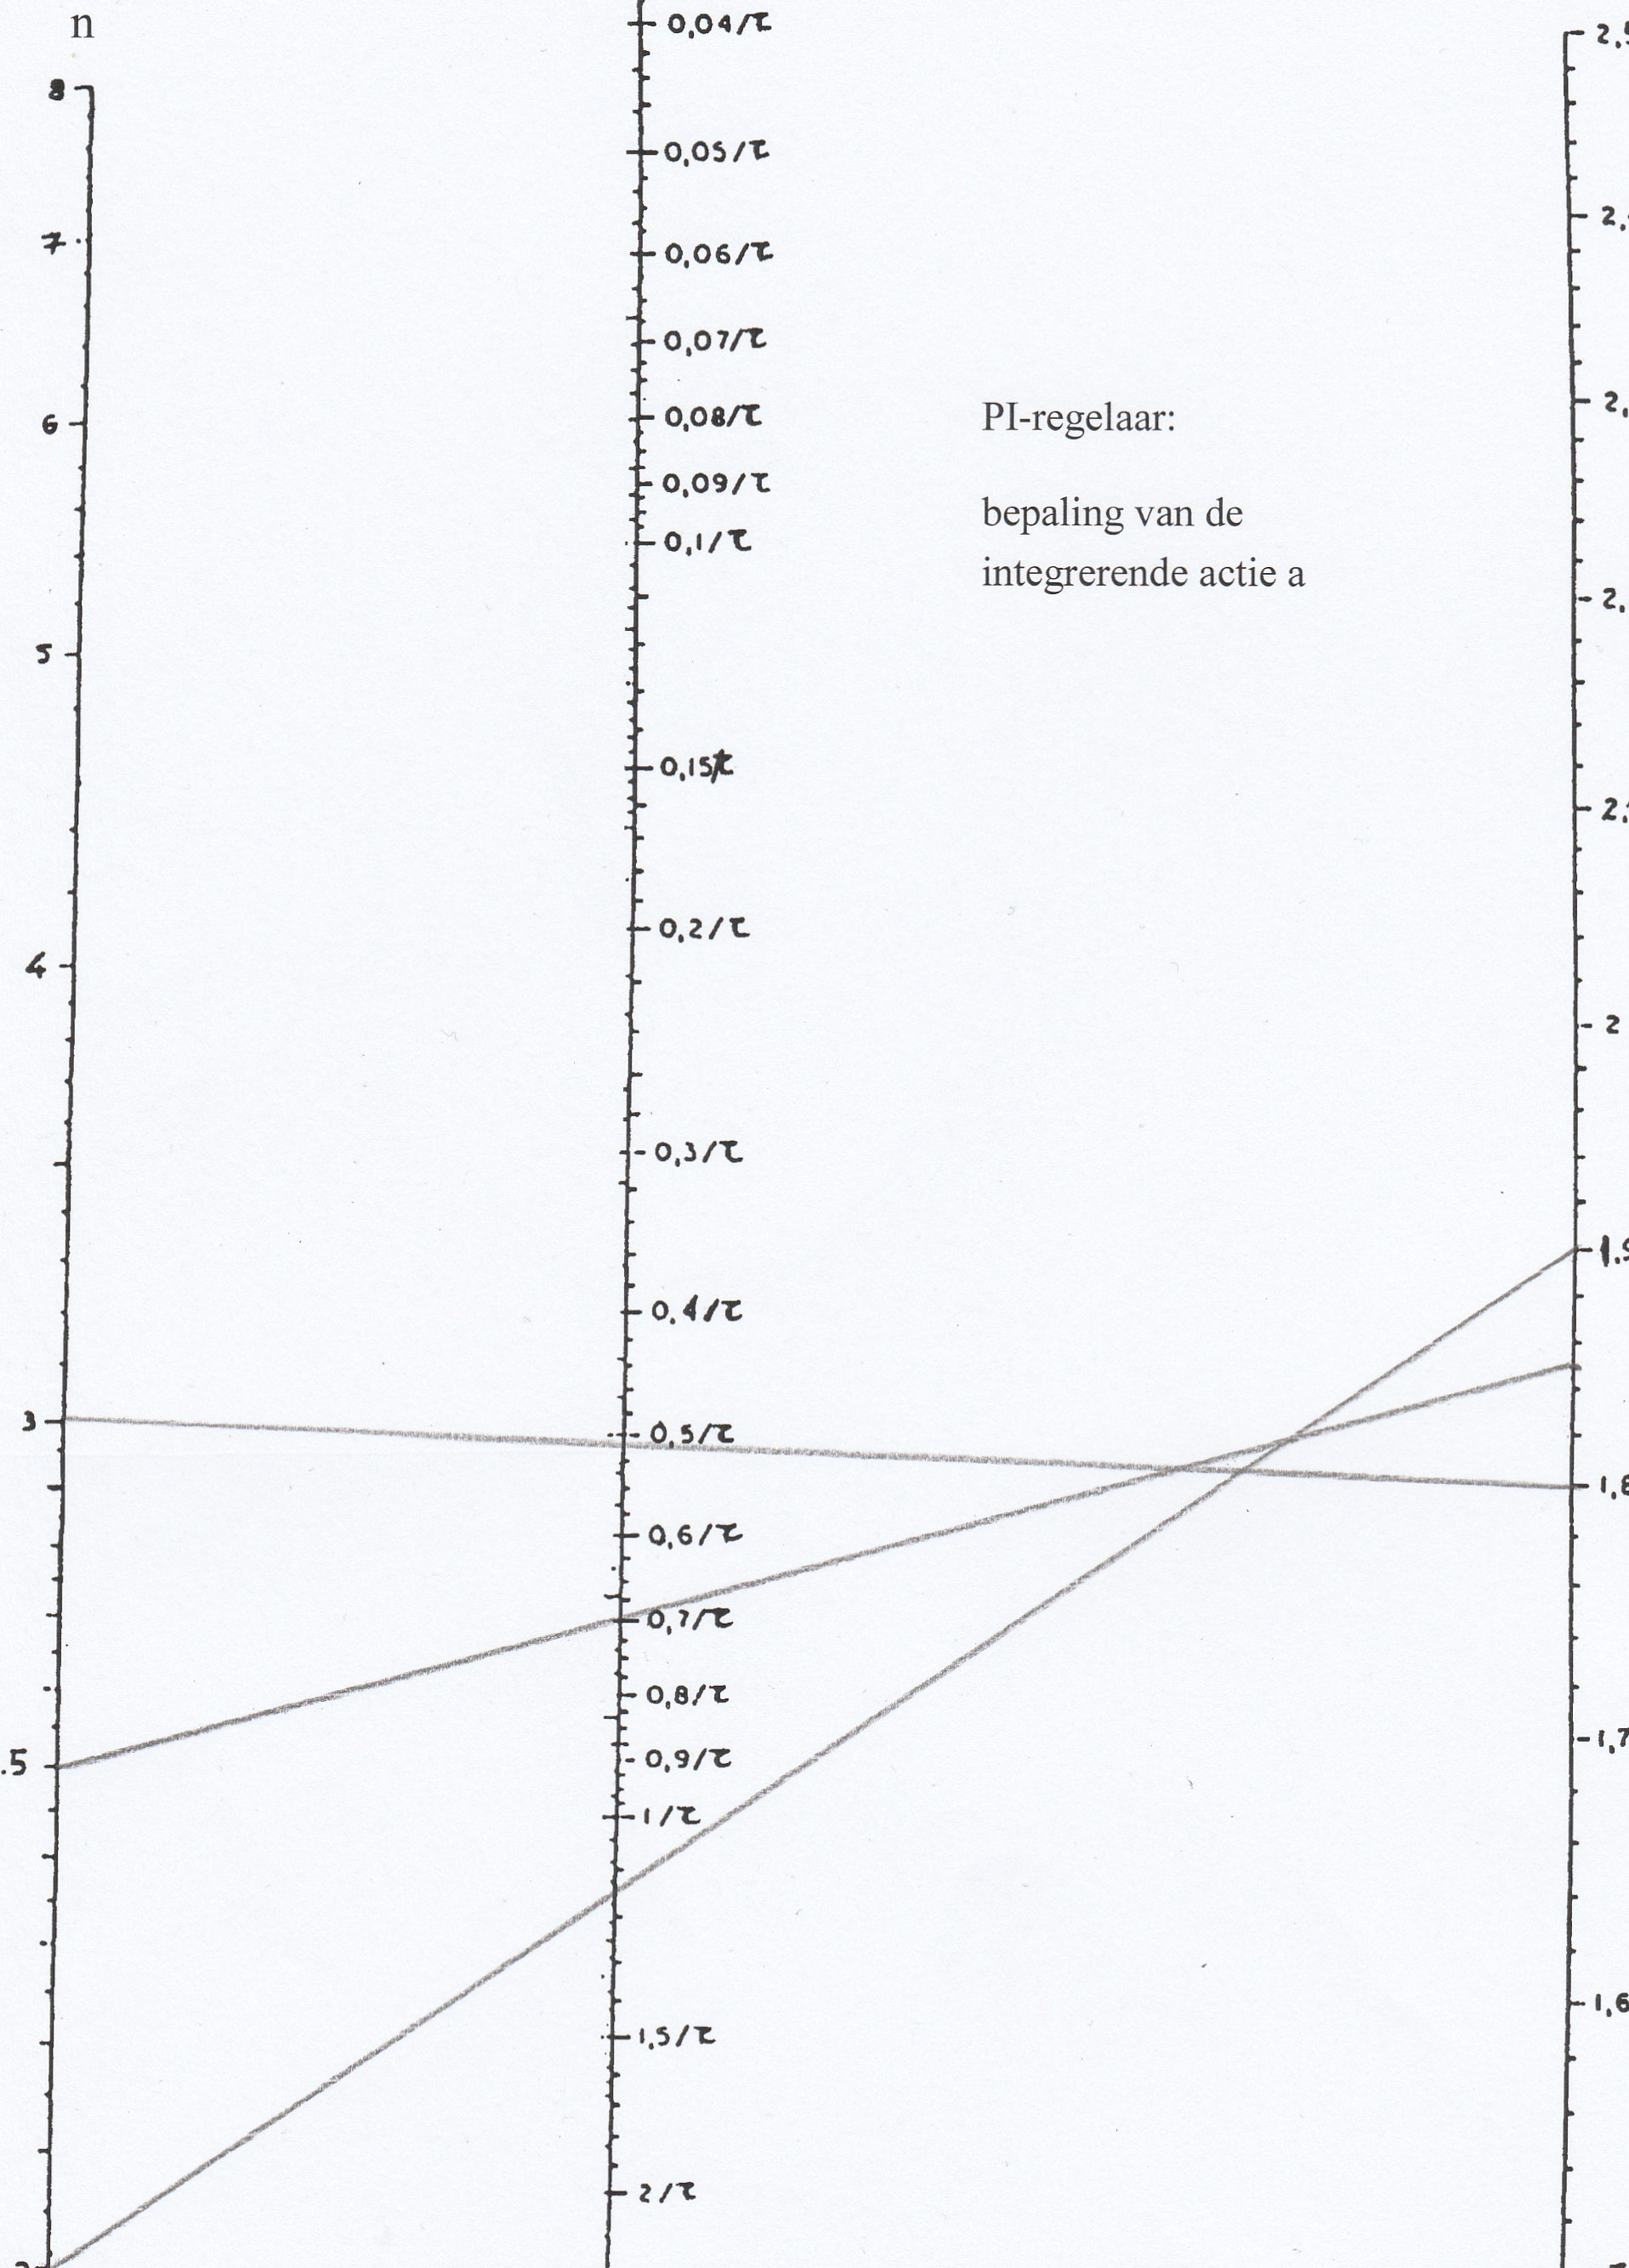
\includegraphics[width=1\linewidth]{Labo2_2_3.jpg}
	\caption{PI-regelaar: bepaling van de integrerende actie a}
	\label{fig:fig2_2_3}
\end{figure}

\subsection{Vergelijk door simulatie zowel de open als de gesloten kringresponsies van model en werkelijk systeem.}


\end{document}
